%%%%%%%%%%%%%%%%%%%%%%%%%%%%%%%%%%%%%%%%%
% Short Sectioned Assignment
% LaTeX Template
% Version 1.0 (5/5/12)
%
% This template has been downloaded from:
% http://www.LaTeXTemplates.com
%
% Original author:
% Frits Wenneker (http://www.howtotex.com)
%
% License:
% CC BY-NC-SA 3.0 (http://creativecommons.org/licenses/by-nc-sa/3.0/)
%
%%%%%%%%%%%%%%%%%%%%%%%%%%%%%%%%%%%%%%%%%

%----------------------------------------------------------------------------------------
%	PACKAGES AND OTHER DOCUMENT CONFIGURATIONS
%----------------------------------------------------------------------------------------

\documentclass[paper=a4, fontsize=11pt]{scrartcl} % A4 paper and 11pt font size

\usepackage[T1]{fontenc} % Use 8-bit encoding that has 256 glyphs
\usepackage{fourier} % Use the Adobe Utopia font for the document - comment this line to return to the LaTeX default
\usepackage[spanish]{babel} % English language/hyphenation
\usepackage[utf8x]{inputenc}
\usepackage{lipsum} % Used for inserting dummy 'Lorem ipsum' text into the template
\usepackage{graphicx}
\graphicspath{ {images/} }
\usepackage{sectsty} % Allows customizing section commands
\allsectionsfont{\centering \normalfont\scshape} % Make all sections centered, the default font and small caps

\usepackage{fancyhdr} % Custom headers and footers
\pagestyle{fancyplain} % Makes all pages in the document conform to the custom headers and footers
\fancyhead{} % No page header - if you want one, create it in the same way as the footers below
\fancyfoot[L]{} % Empty left footer
\fancyfoot[C]{} % Empty center footer
\fancyfoot[R]{\thepage} % Page numbering for right footer
\renewcommand{\headrulewidth}{0pt} % Remove header underlines
\renewcommand{\footrulewidth}{0pt} % Remove footer underlines
\setlength{\headheight}{13.6pt} % Customize the height of the header


%\setlength\parindent{0pt} % Removes all indentation from paragraphs - comment this line for an assignment with lots of text

%----------------------------------------------------------------------------------------
%	TITLE SECTION
%----------------------------------------------------------------------------------------

\newcommand{\horrule}[1]{\rule{\linewidth}{#1}} % Create horizontal rule command with 1 argument of height

\title{	
\normalfont \normalsize 
\textsc{Universidad de Castilla La Mancha} \\ [25pt] % Your university, school and/or department name(s)
\horrule{0.5pt} \\[0.4cm] % Thin top horizontal rule
\huge Artículo 3. Using OLAP and multidimensional data for decision making \\ % The assignment title
\horrule{2pt} \\[0.5cm] % Thick bottom horizontal rule
}

\author{José María García García} % Your name

\date{\normalsize\today} % Today's date or a custom date

\begin{document}

\maketitle % Print the title

%----------------------------------------------------------------------------------------
%	PROBLEM 1
%----------------------------------------------------------------------------------------

\section{Preguntas}

Leer el artículo y obtener de él información acerca de los siguientes puntos.

\begin{itemize}
\item \textbf{ ¿Qué dos sistemas puede utilizar un gestor para obtener un mejor conocimiento de su empresa?}
\end{itemize}
Procesamiento analítico en línea y Bases de Datos de Múltiples Dimensiones. Estos sistemas nos presentan información resumida que han extraído de las bases de la empresa. Cogen datos sobre el rendimiento de la empresa, los trocean y organizan en estructuras de varias dimensiones y los presentan de manera que permite a los gestores descubrir problemas más rápidamente. 

\begin{itemize}
\item \textbf{¿Qué diferencia hay entre los sistemas OLTP y OLAP?}
\end{itemize}
Los sistemas OLTP son sistemas de procesamiento de transacciones en línea, por lo que están centrados en las operaciones del día a día de la empresa, y no tanto en el análisis de los datos que generan esas transacciones. No obstante, estos sistemas suelen incorporar mecanismos para generar informes según las actividades de la empresa, pero estos no sirven para tener una visión general ni para apreciar rápidamente puntos fuertes y puntos débiles. 

\begin{itemize}
\item \textbf{A la hora de obtener información sobre el funcionamiento general de la empresa, ¿qué características tiene el tipo de sistema preferido 	 por los gestores?}
\end{itemize}
A diferencia del sistema comentado anteriormente, un sistema que usa OLAP y MDDB es intuitivo, fácil de usar y está orientado a la busqueda de información de tal forma que permita, mediante un vistazo rápido, saber que está pasando en la empresa y formarse una idea general sobre la misma.
	
\begin{itemize}
\item \textbf{¿Cómo se representa la información cuando utilizamos una base de datos multidimensional?. Indica un ejemplo}
\end{itemize}

\begin{figure}
\centering
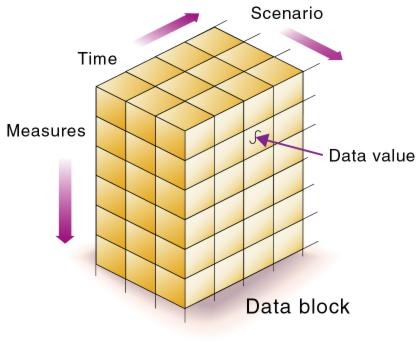
\includegraphics{cubo}
\end{figure}

\begin{itemize}
\item \textbf{¿Cómo es el proceso de implantación de un ERP?}
\end{itemize}

\begin{itemize}
\item \textbf{¿Cómo es el proceso de implantación de un ERP?}
\end{itemize}

%------------------------------------------------



\section{Lists}

%------------------------------------------------

\subsection{Example of list (3*itemize)}

%------------------------------------------------

\subsection{Example of list (enumerate)}
\begin{enumerate}
\item First item in a list 
\item Second item in a list 
\item Third item in a list
\end{enumerate}

%----------------------------------------------------------------------------------------

\end{document}